\documentclass{article}

\usepackage{graphicx}
\usepackage{amsmath}
\usepackage{xepersian}

\settextfont{Times New Roman}

\title{تمرین دوم طراحی سیستم‌های دیجیتال}
\author{پارسا محمدیان -- 98102284}

\begin{document}
\maketitle
\newpage
\section*{محسابه تأخیر به صورت تئوری}
در طراحی جمع‌کننده 4 بیتی، 4 عدد 
\lr{Full Adder}
به صورت آبشاری به یکدیگر بسته شده‌اند. 
پس برای محاسبه تأخیر هر خروجی نیاز است که تأخیر هر 
\lr{Full Adder}
را جمع کنیم (شکل \ref{FourBitAdderDelay}).
تأخیر هر 
\lr{Full Adder}
را نیز می‌توانیم از تأخیر 
\lr{Half Adder}
که مشخص است محاسبه کنیم (شکل \ref{FADelay}).

\begin{figure}[!htbp]
    \centering
    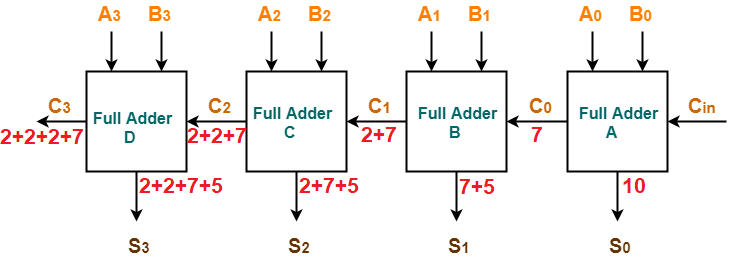
\includegraphics[width=\linewidth]{FourBitAdderDelay.png}
    \caption{تأخیر \lr{Four Bit Adder}}
    \label{FourBitAdderDelay}
\end{figure}

\begin{figure}[!htbp]
    \centering
    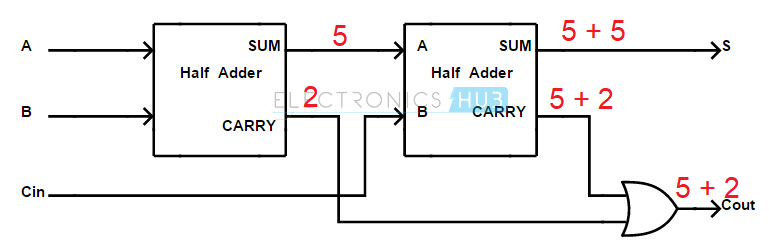
\includegraphics[width=\linewidth]{FADelay.png}
    \caption{تأخیر \lr{Full Adder}}
    \label{FADelay}
\end{figure}

\begin{latin}
\begin{gather*}
    \text{HA}
    \begin{cases}
        \text{Delay(sum) = 5}\\
        \text{Delay(carry) = 2}
    \end{cases} \\
    \text{FA}
    \begin{cases}
        \text{Delay(sum) = 10}\\
        \text{Delay(carry) = 7}
    \end{cases} \\
    \text{FourBitAdder}
    \begin{cases}
        \text{Delay(sum) = 16}\\
        \text{Delay(carry) = 13}
    \end{cases}
\end{gather*}
\end{latin}

پس به صورت تئوری جمع‌کننده 4 بیتی طراحی شده تأخیر 16 واحد زمانی برای 
\lr{sum}
و 13 واحد زمانی برای 
\lr{carry}
دارد.

\section*{محاسبه تأخیر به وسیله‌ی \lr{ModelSim}}
برای محاسبه تأخیر به وسیله‌ی 
\lr{ModelSim} 
ابتدا دو ورودی نمونه مناسب برای حداکثر تأخیر انتخاب می‌کنیم. در اینجا دو عدد 
1010
و
0101
را با رقم نقلی ورودی 1 جمع زده‌ام. تأخیر را می‌توان از شکل موج 
(\lr{Wave Form})
خواند.

همانطور که در شکل
\ref{ModelSim}
نشان داده شده، تأخیر محاسبه شده در قسمت قبلی کاملا دقیق است.

\begin{figure}[!htbp]
    \centering
    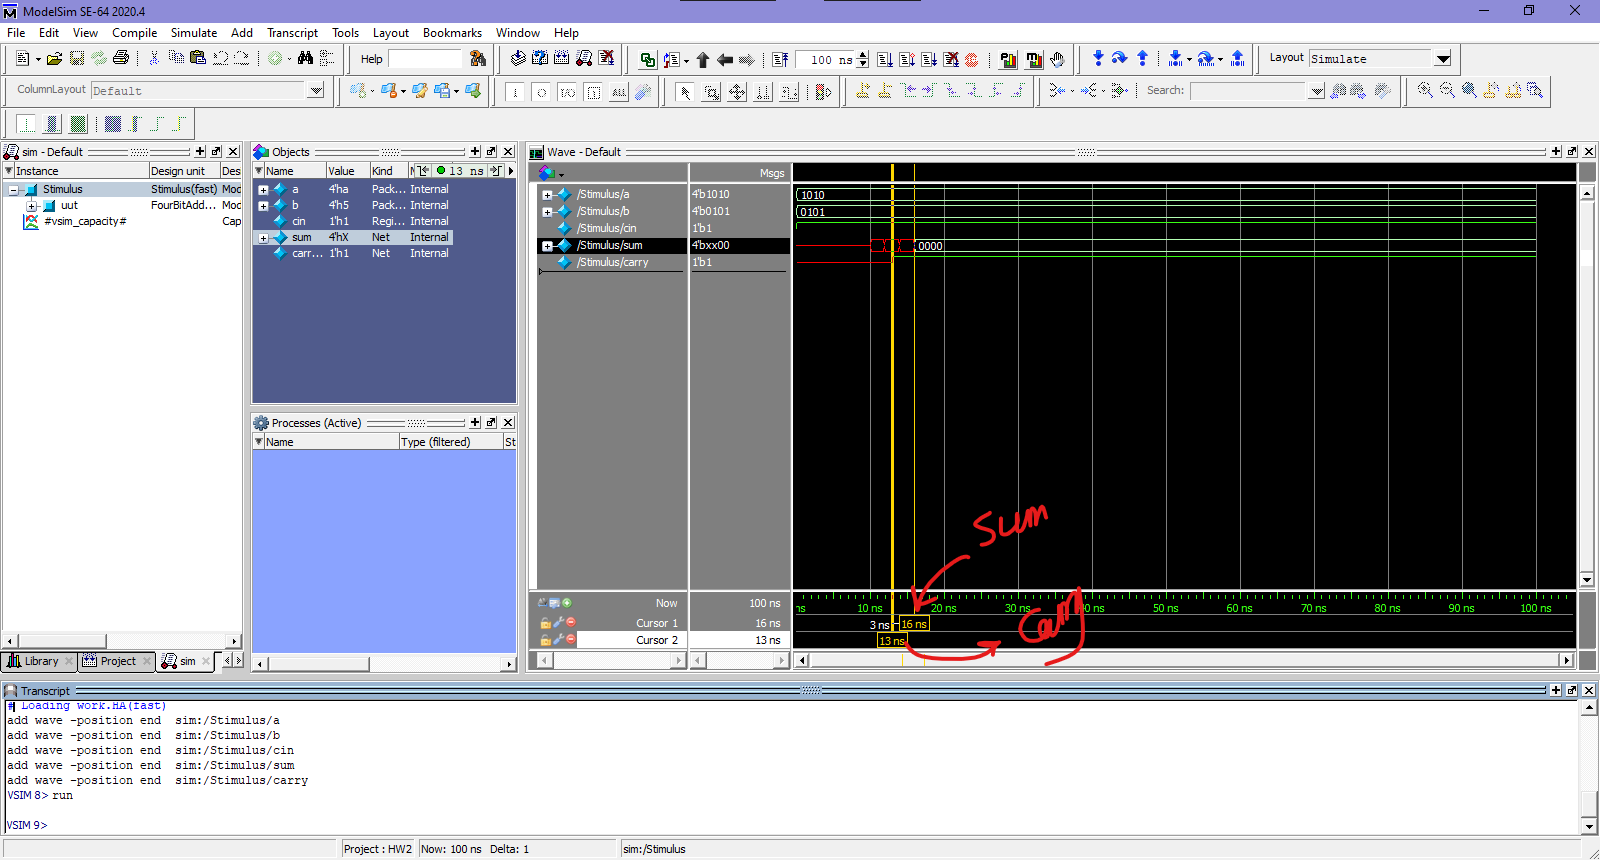
\includegraphics[width=\linewidth]{ModelSim.png}
    \caption{تأخیر \lr{ModelSim}}
    \label{ModelSim}
\end{figure}

\end{document}